\chapter{Gamma detection testing}



\section{Photodiodes testing}

\section{Detection test of the Co$^{57}$ spectra}



\subsection*{•}

\subsection*{•}

\subsection*{•}


\section{Noise and its reduction}
The measured spectra are affected by noise. In order to reduce noise,  two - the detector  
\subsection{Electromagnetic noise reduction}
Photodiodes have to be sufficiently electromagnetically shielded and their distance to the preamplifier input should be as short as possible. 


\begin{figure}[H]
 \centering
 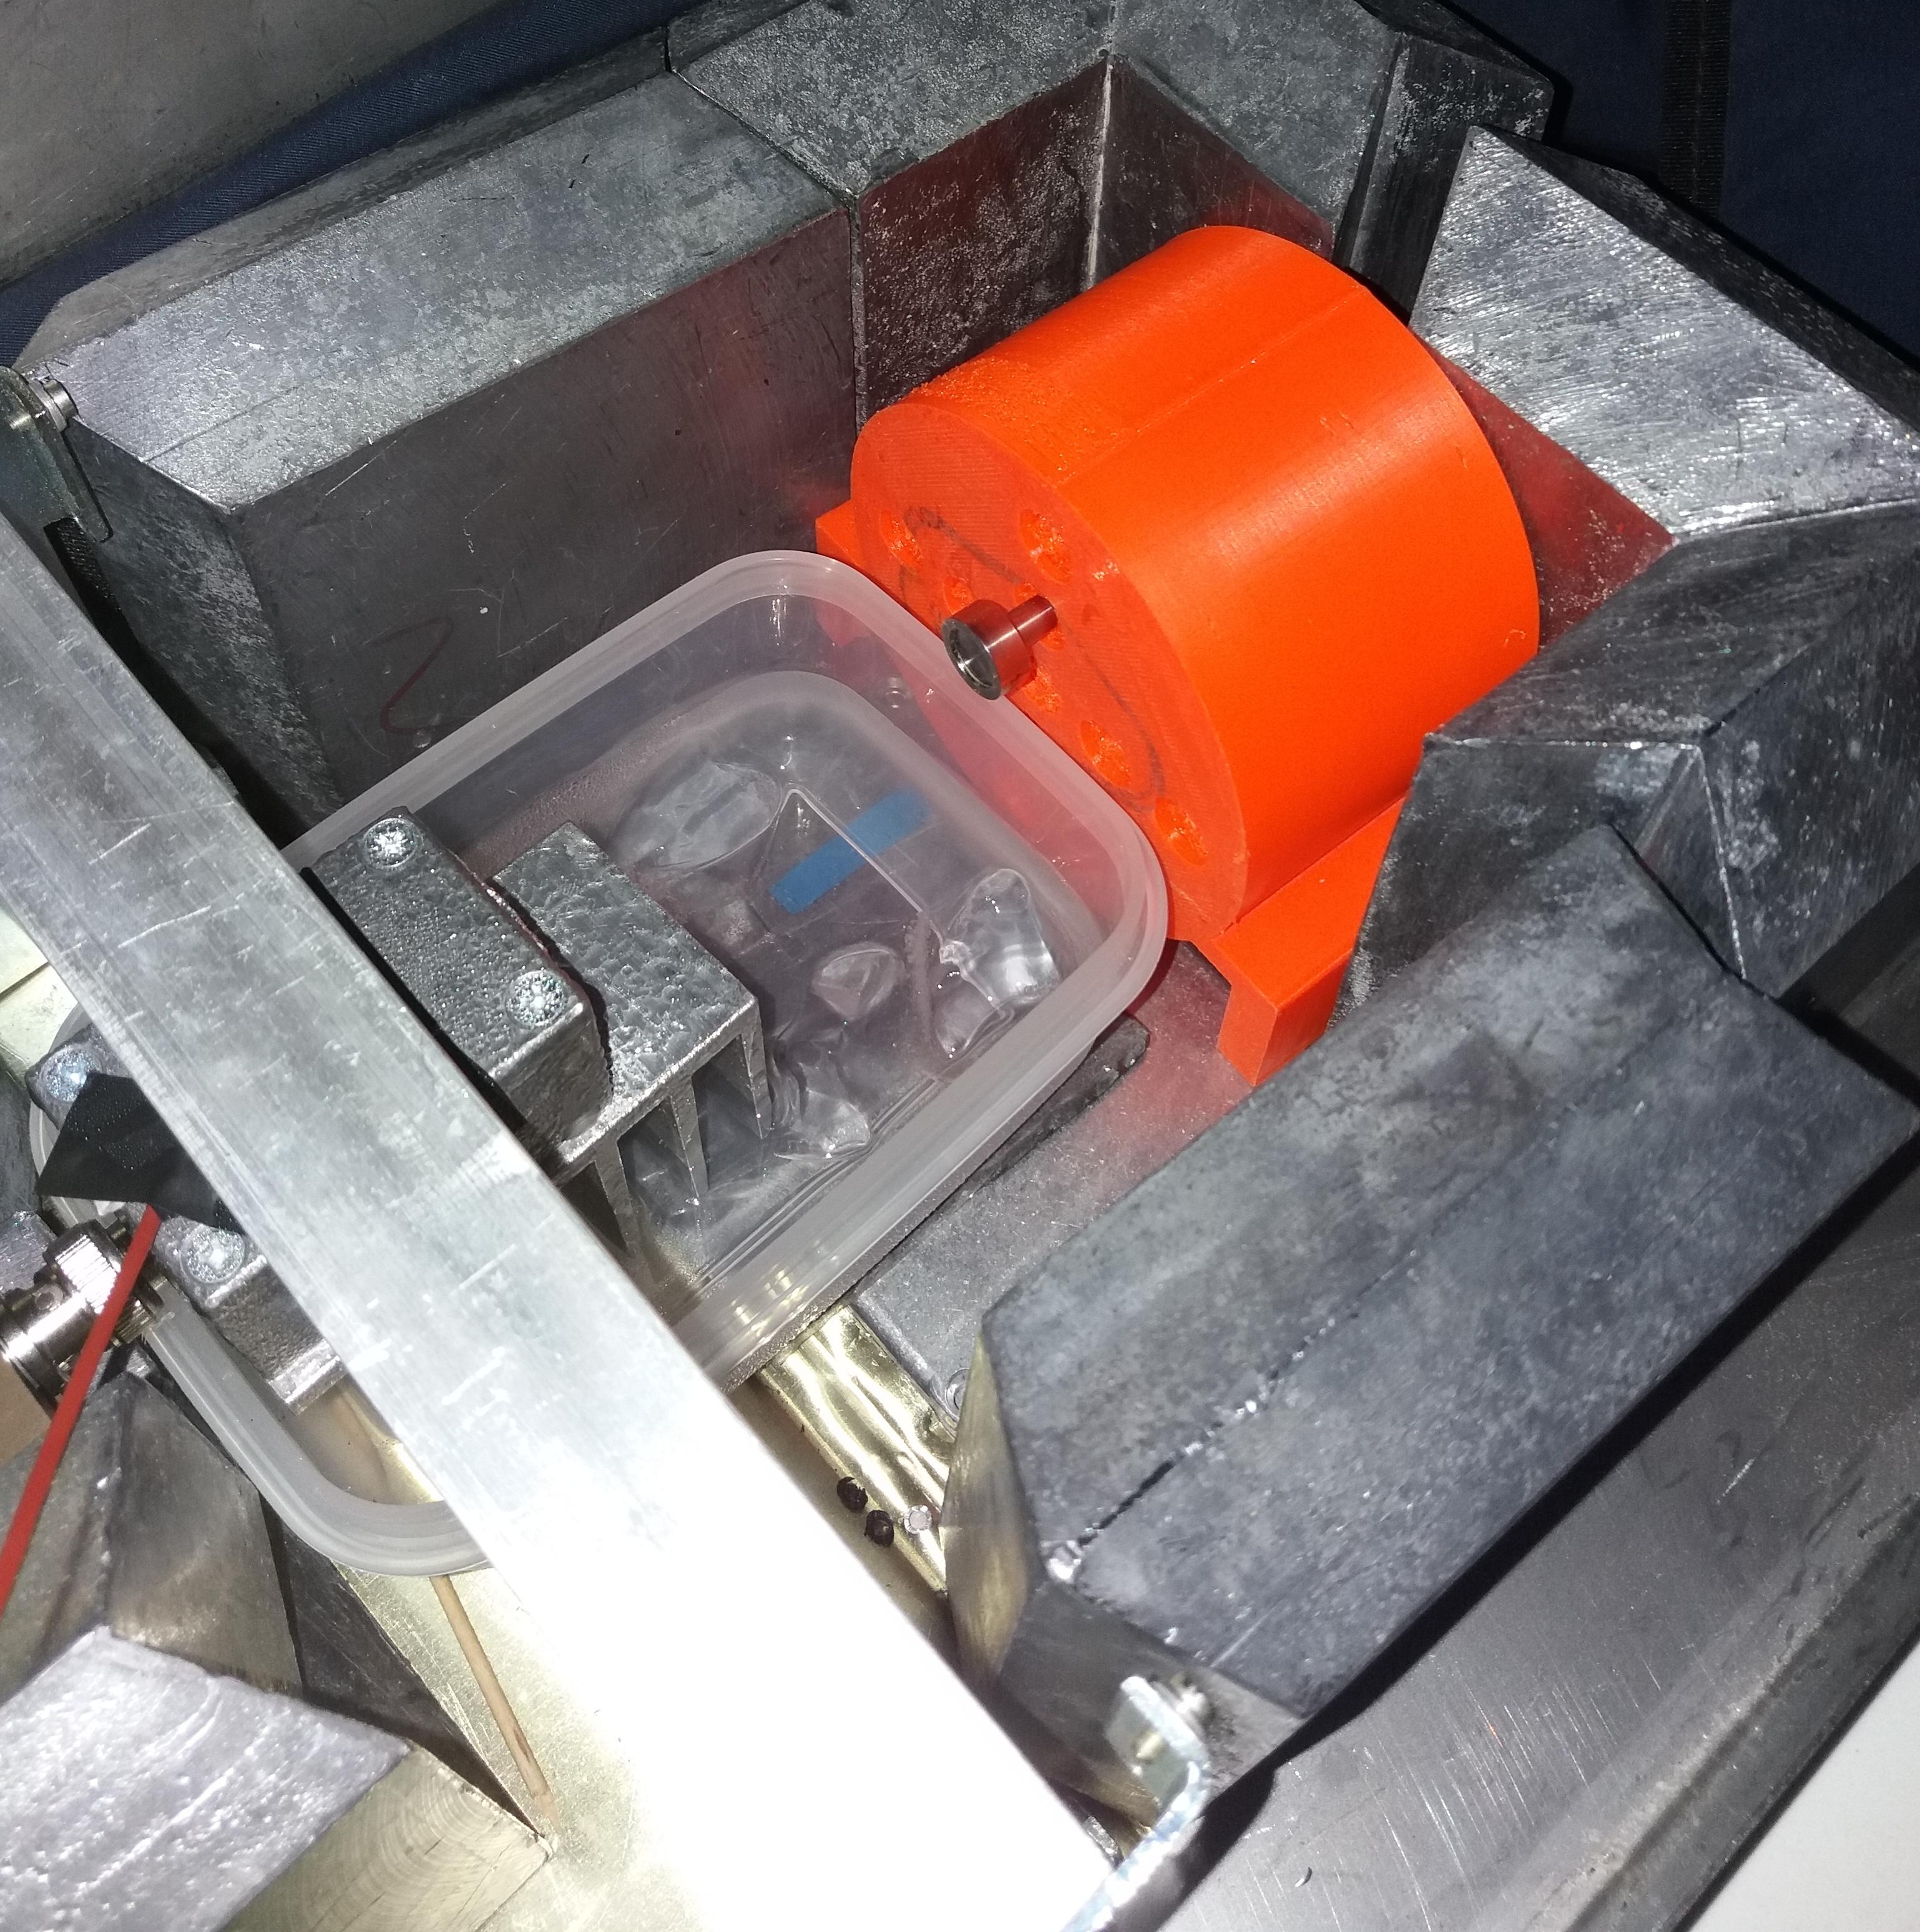
\includegraphics[scale=0.09, angle = 0]{./pictures/chlazeniLedem.jpg}
 \caption{Example of Co$^{57}$ spectra from poorly shielded detector setup.}
 \label{notShielded}
 
\end{figure}



\subsection{Thermal noise reduction}
To reduce the thermal noise, the S14605 photodiode was cooled by ice. It was placed in shielding box, which had attached heat sink to the bottom. This heat sink was submerged into the small tub filled with a melting ice (picture \ref{cooler}). The thermal conduction was improved by sticking the photodiode to the of the floor of the shielding box by conduction paste. The photodiode was cooled this way to temperatures around 7-8 $^\circ$C.


\begin{figure}[H]
 \centering
 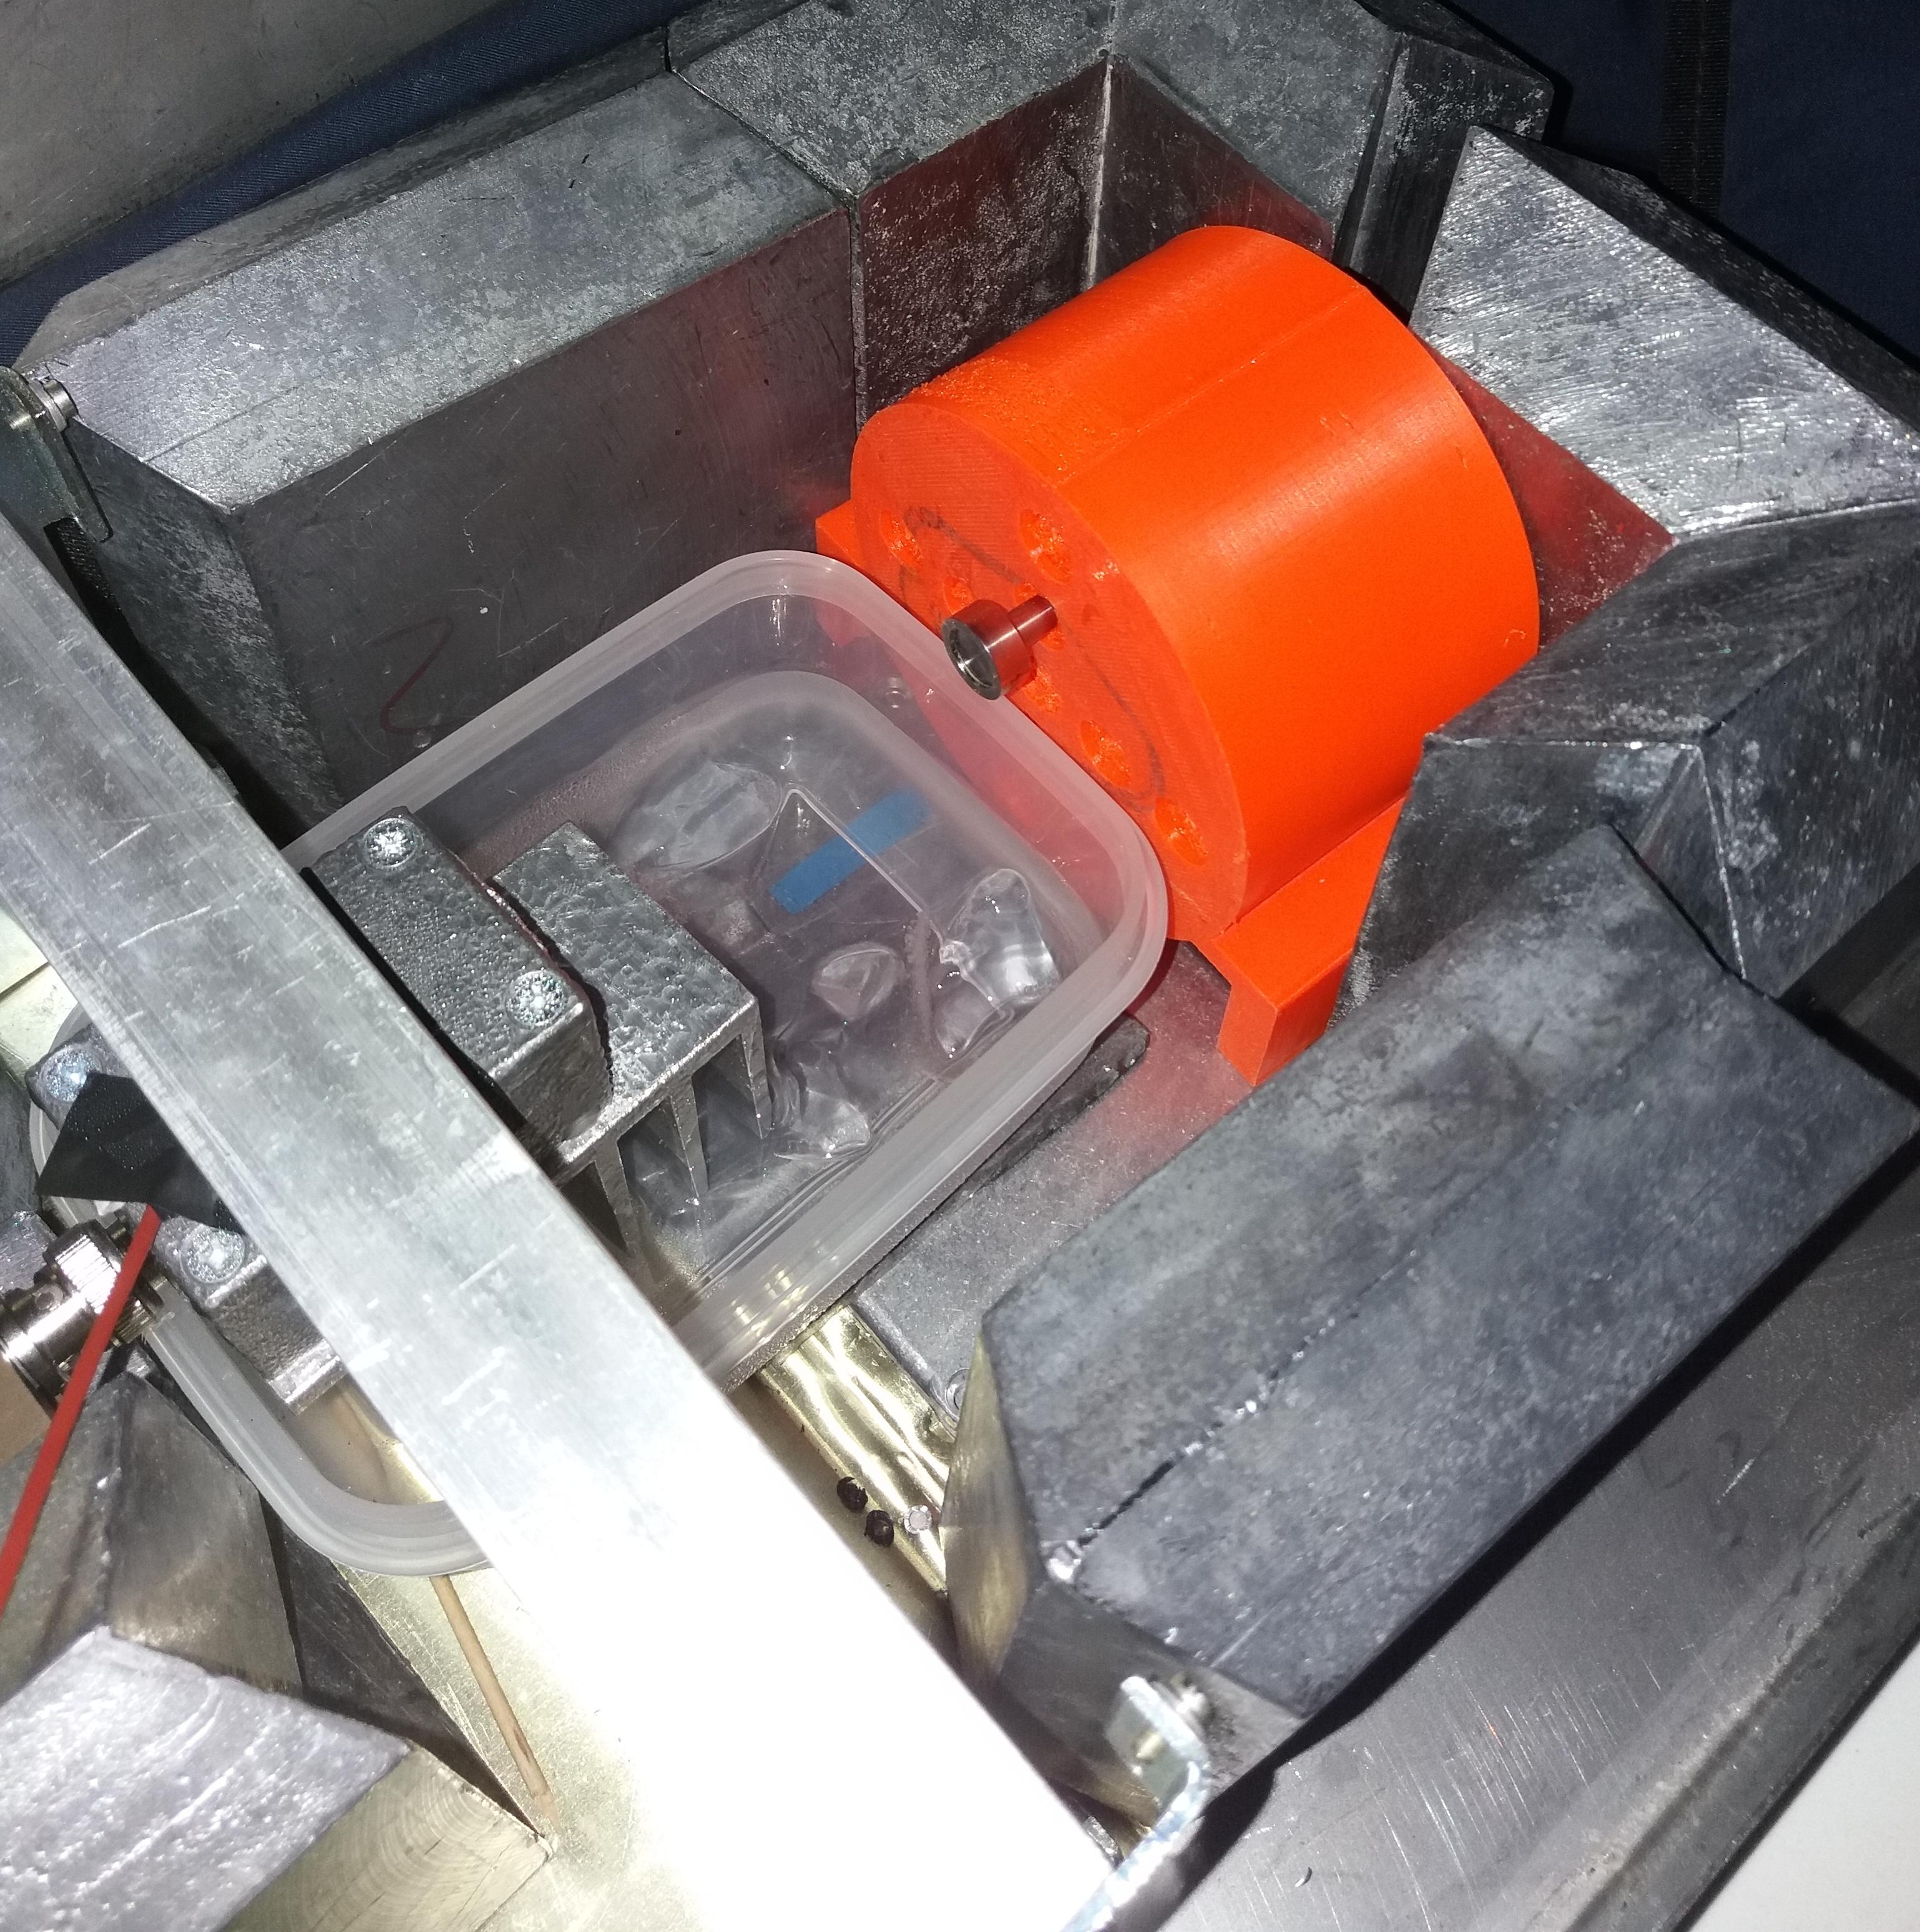
\includegraphics[scale=0.09, angle = 0]{./pictures/chlazeniLedem.jpg}
 \caption{Detector cooled by ice.}
 \label{cooler}
 
\end{figure}



\begin{figure}[H]
 \centering
 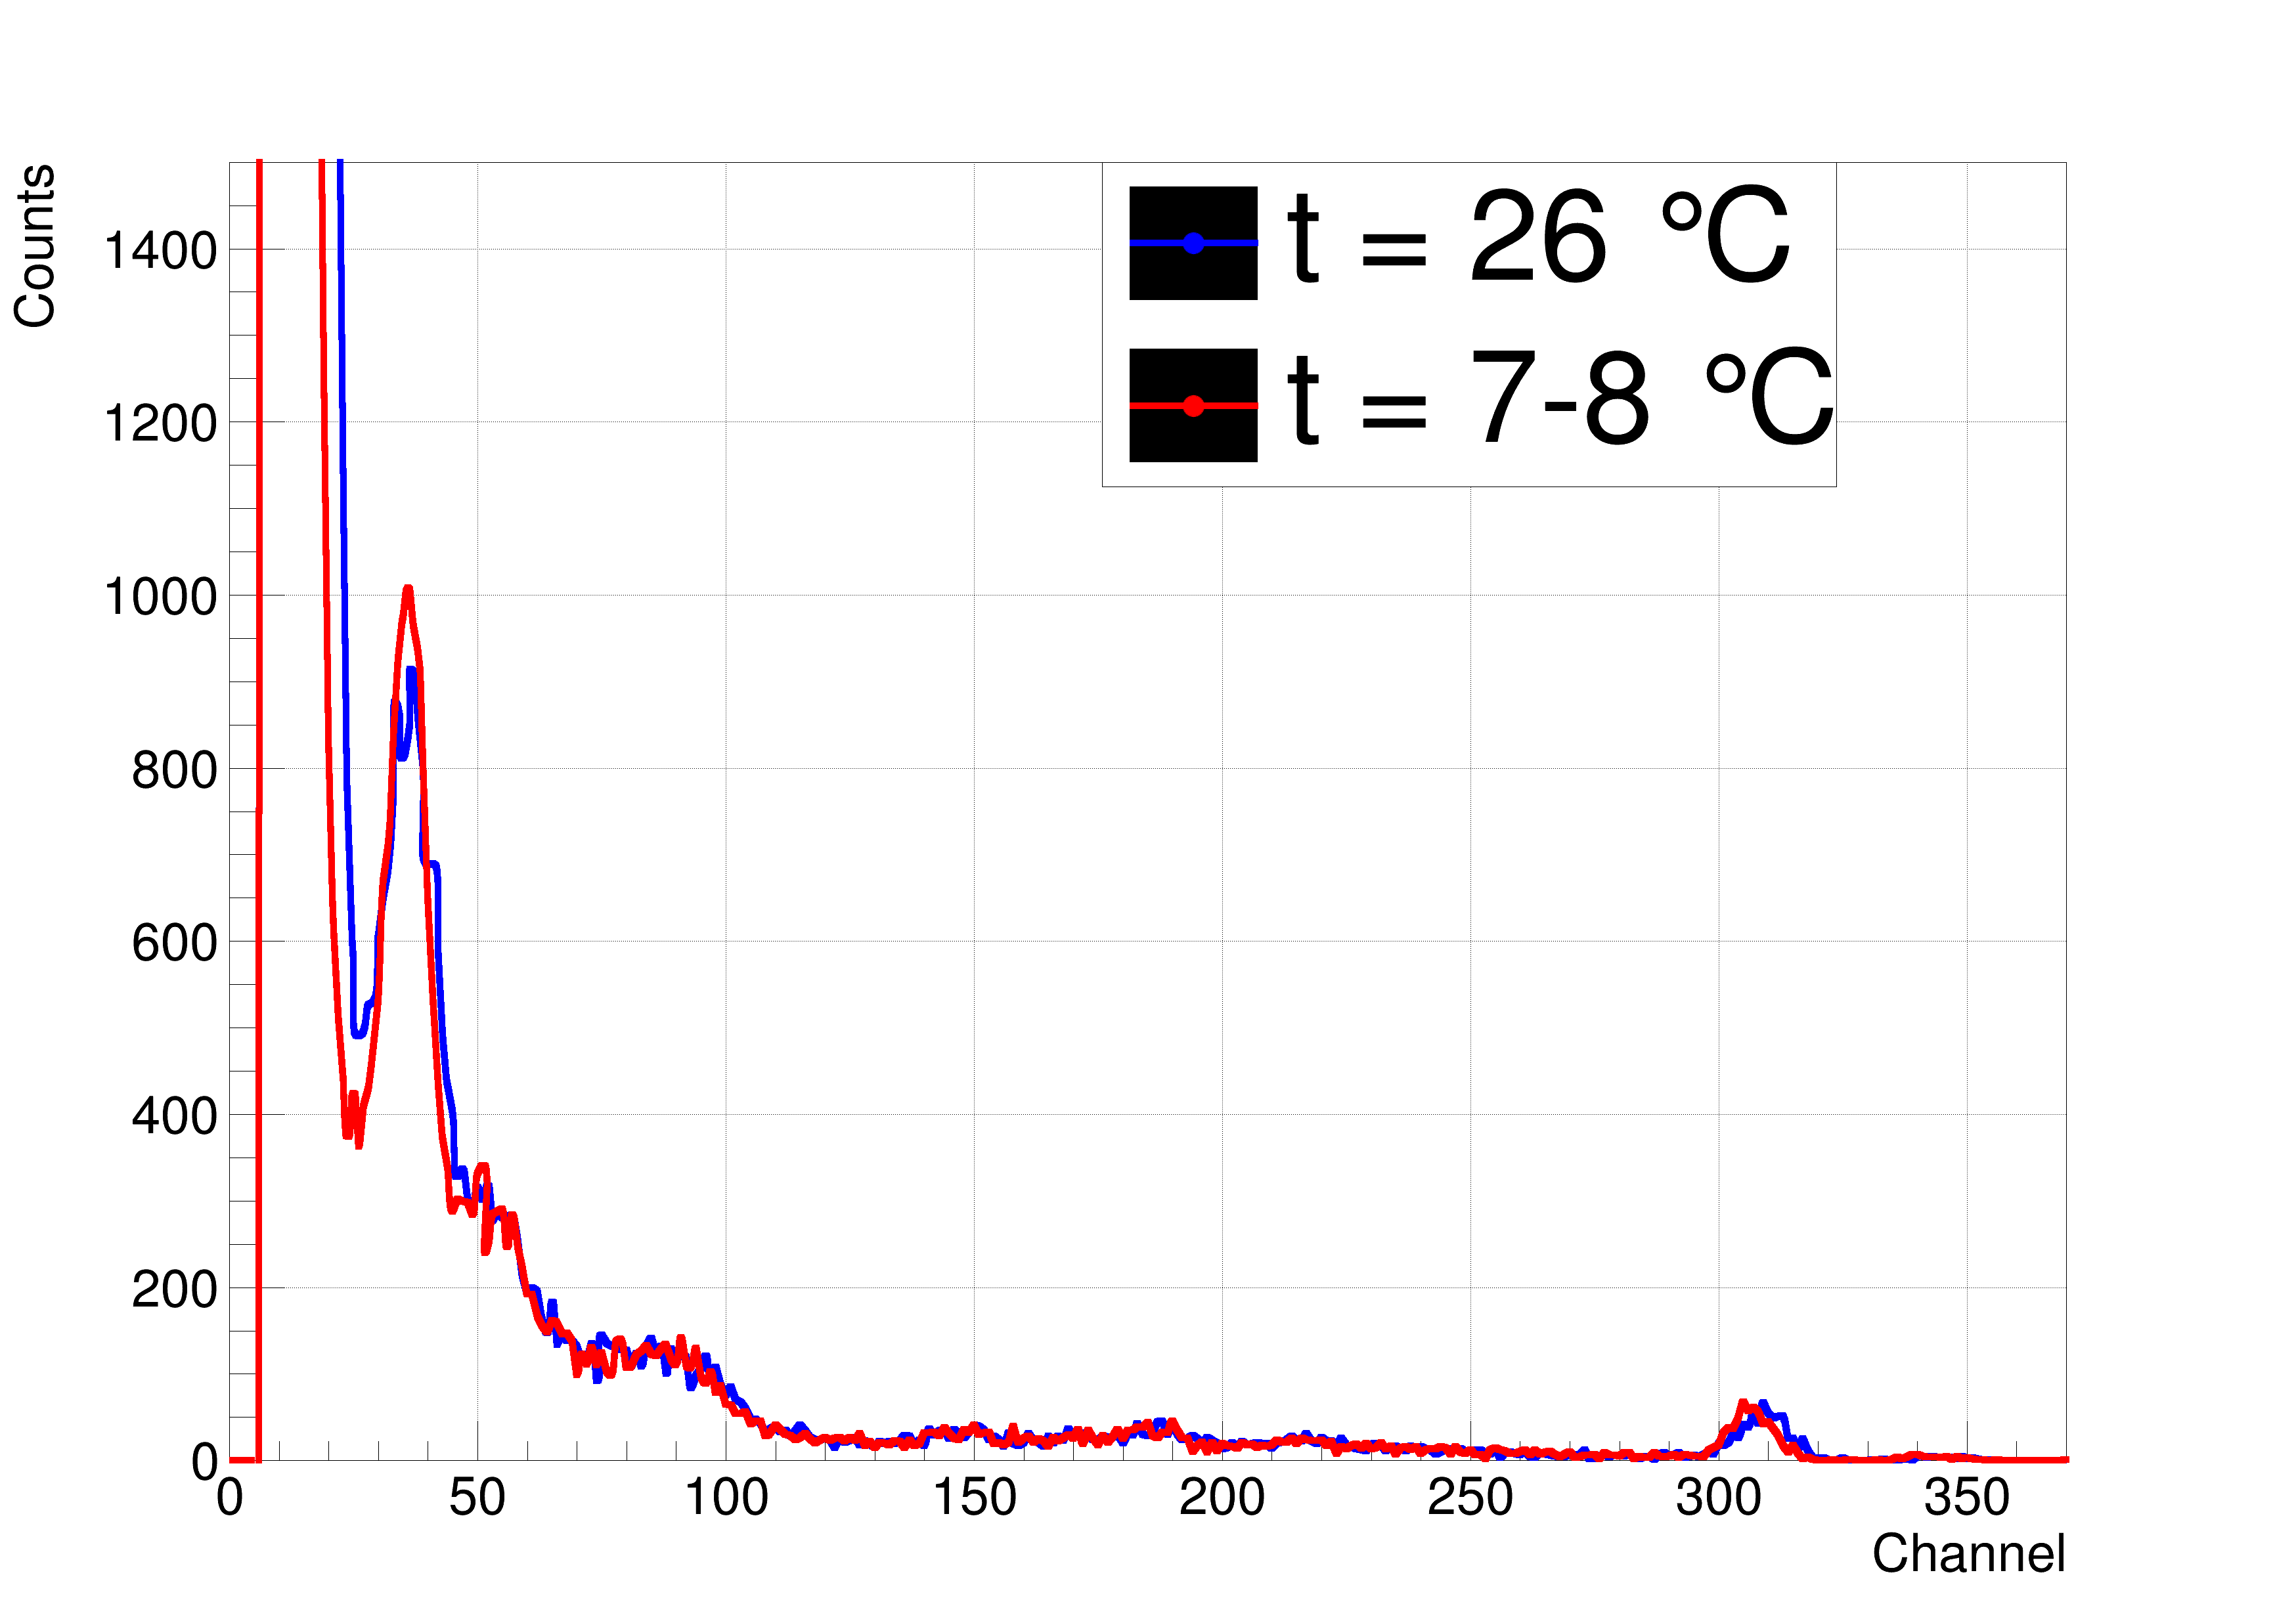
\includegraphics[scale=0.13, angle = 0]{./pictures/TempDiff.png}
 \caption{Measured Co$^{57}$ spectra at two different temperatures.}
 \label{coolspectr}
 
\end{figure}








\par
The results show that the cooling improves SNR, but this effect is small when compared to the effect of shielding. It was also tried to use the peltier cooler instead, however, the cooling efficiency was low when compared to the ice.
